%! TeX program = lualatex
\documentclass[twoside, openany, a4paper, 12pt]{book}

\title{Wstęp do teorii reprezentacji}
\author{\color{subtext1}Weronika Jakimowicz}
\date{
  Lato 2025/26\bigskip\\ 
  \small\slshape\color{subtext1}
  Notatki i myśli własne do wykładu prof. Marka Bożejki oraz ćwiczeń prof. Jana Dymary.
}

\usepackage[pl]{../../template}

\usepackage{halloweenmath}

\let\oldamalg\amalg
\newcommand{\uu}[1]{\underline{#1}}
\newcommand{\Mm}{\ensuremath{\mathfrak{M}}}
\newcommand{\lr}{\leftrightarrow}

\DeclareMathOperator{\Cn}{Cn}
\DeclareMathOperator{\Th}{Th}

\DeclareMathOperator{\Hh}{\mathcal{H}}
\DeclareMathOperator{\U}{\mathcal{U}}
\DeclareMathOperator{\B}{\mathcal{B}}


\begin{document}
\frontmatter 
\maketitle
\thispagestyle{empty}
\setcounter{page}{0}

\tableofcontents
\mainmatter

\pagestyle{fancy}

\chapter{Szybki kurs matematyki}  

\section{O grupach krótko}

Grupa jaka jest każdy wie. Nas ostatecznie będą interesowały grupy zwarte i lokalnie zwarte. Najpierw ujednorodnijmy wiedzę z algebry.

\subsection{Grupy wolne}

Grupa wolna $F_S$ o generatorach $S$ to zbiór ciągów elementów z $S\cup S^{-1}$ gdzie jedyne skrócenia jakie akceptujemy to $ss^{-1}$ dla $s\in S$.

\begin{example}[m]
  \item Liczby całkowite $\Z$ tworzą grupę wolną o jednym generatorze.
  \item Grupę $F_2$ o generatorach $s$, $t$ można przedstawić jako nieskończone drzewo $4$-regularne. Wtedy elementy $F_2$ to ścieżki startujące w pewnym wyróżnionym wierzchołku.
    \begin{center}
      
\begin{tikzpicture}[thick, cap=round]
        \draw (-2,0)--(2,0);
        \draw (0,-2)--(0,2);
        
        \draw (-1,-.75)--(-1,.75);
        \draw (1,-.75)--(1,.75);
        \draw (-.75,1)--(.75,1);
        \draw (-.75,-1)--(.75,-1);

        \draw (-1.5,.3)--(-.5,.3);
        \draw (-1.5,-.3)--(-.5,-.3);
        \draw (1.5,-.3)--(.5,-.3);
        \draw (1.5,.3)--(.5,.3);

        \draw (-.3, .5)--(-.3,1.5);
        \draw (.3, .5)--(.3,1.5);
        \draw (-.3, -.5)--(-.3,-1.5);
        \draw (.3, -.5)--(.3,-1.5);
      \end{tikzpicture}
    \end{center}
\end{example}

\begin{lemma}{}{}
  Każda grupa $G$ jest obrazem pewnej grupy wolnej $F_S$ dla pewnego zbioru generatorów $S$.
\end{lemma}

\begin{definition}{prezentacja grupy}{}
  Niech $S$ będzie zbiorem generatorów z lematu wyżej, a $R$ - jądrem homomorfizmu $G\to F_S$. Wtedy $\langle S|R\rangle$ nazywamy \textbf{prezentacją grupy $G$}, gdzie $S$ to jej generatory, a $R$ - relacje.
\end{definition}

\begin{example}
Grupa $S_3$ permutacji zbioru trzyelemntowego ma prezentację 
$$\langle \sigma_1, \sigma_2|\sigma_1^2=\sigma_2^1=(\sigma_1\sigma_2)^3=id\rangle,$$ 
gdzie $\sigma_i$ to permutacja $(i, i+1)$.
\end{example}

Powstaje pytanie jak sprawdzać, czy dana podgrupa $H\leq G$ jest wolna. Na przykład czy podgrupa
$$H=\left\langle\begin{bmatrix}1&2\\0&1\end{bmatrix},\begin{bmatrix}1&0\\2&1\end{bmatrix}\right\rangle\leq SL_2(\R)$$ 
generują podgrupę wolną. Z pomocą przychodzi lemat o ping pongu, który w najprostszej wersji mówi:

\begin{lemma}{ping pong}{}
  Niech $a, b\in G$ będą elementami grupy działającej na pewnym zbiorze $X$. Jeśli istnieją niepuste, rozłączne podzbiory $A,B\subseteq X$ takie, że dla wszystkich $n\in \N$ $a^nB\subseteq A$ oraz $b^nA\subseteq B$ to podgrupa $\langle a,b\rangle$ jest wolna.
\end{lemma}

\begin{proof}
  Weźmy dowolne słowo $w=a^{n_k}b^{m_k}...a^{n_1}b^{m_1}$ w skróconej postaci. 

  Na początek załóżmy, że $n_1$ oraz $n_k$ nie są zerowe oraz $m_k=0$. Wtedy dla $x\in B$ gramy w ping ponga idąc od końca słowa $w$. $a^{n_k}x\in A$, więc $b^{n_{k-1}}(a^{n_k}x)\in B$ i tak dalej aż dochodzimy do $b^{m_1}...a^{n_k}x\in B$, które $a^{n_1}$ wrzuca z powrotem w $A$. Ponieważ $A\cap B=\emptyset$ to $A\ni wx\neq x\in B$, czyli $w\neq 1$. 

  Pozostaje nam rozważyć przypadek, kiedy słowo zaczyna się literką $a$ i kończy literką $b$, czyli jest postaci $w=a^n w'b^m$. Załóżmy nie wprost, że $a^nw'b^m=1$, wtedy $a^n(a^nw'b^m)a^{-n}=a^n1a^{-n}=1$, ale $a^{2n}w'b^ma^{-n}$ jest słowem zaczynającym i kończącym się potęgą litery $a$ - dostajemy sprzeczność z rozumowaniem wyżej.
\end{proof}

Ćwiczenie dla studenta: jak uogólnić powyższy lemat by sprawdzać, czy $\langle a_1,...,a_n\rangle\leq G$ jest grupą wolną?

\subsection{Graf Cayley'a}

\begin{definition}{graf Cayley}{}
  Niech $G=\langle S|R\rangle$ będzie prezentacją grupy. Graf Cayley dla zbioru generatorów $S$ definiujemy jako skierowany graf $\Gamma(G, S)$ gdzie
  \begin{itemize}
    \item wierzchołki to elementy grupy $V=G$
    \item a krawędzie to przesunięcia o generator lub jego odwrotność, $E=\{(v,vs)\;:\;v\in G, s\in S\cup S^{-1}\}$.
  \end{itemize}
\end{definition}

Z racji że z każdego wierzchołka grafu Cayley wyprowadzamy po jednej krawędzi dla każdego generatora, to jest on zawsze $|S|$-regularny oraz spójny.

\begin{example}
  Rozważmy grupę $S_3=\langle \sigma_1, \sigma_2|\sigma_1^2=\sigma_2^2=(\sigma_1\sigma_2)^3\rangle$. Wtedy jej graf Cayley to 
  \begin{center}
    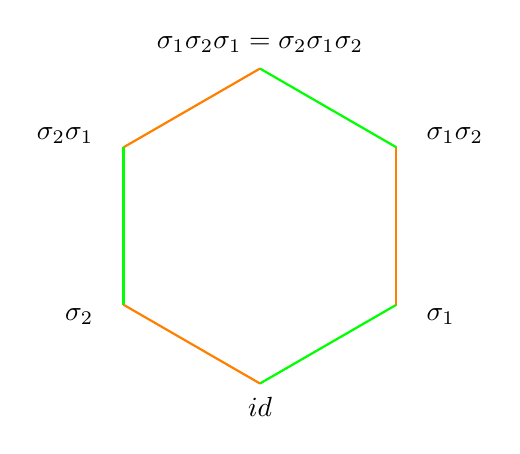
\begin{tikzpicture}
      \foreach \i in {0,2,4} {
        \draw[green, thick] ({-90+\i*60}:2)--({-90+(\i+1)*60}:2);
        \draw[orange, thick] ({-30+\i*60}:2)--({-30+(\i+1)*60}:2);
      }

      \node at (-90:2.3) {$id$};
      \node[anchor=west] at (-30:2.3) {$\sigma_1$};
      \node[anchor=west] at (30:2.3) {$\sigma_1\sigma_2$};
      \node at (90:2.3) {$\sigma_1\sigma_2\sigma_1=\sigma_2\sigma_1\sigma_2$};
      \node[anchor=east] at (150:2.3) {$\sigma_2\sigma_1$};
      \node[anchor=east] at (-150:2.3) {$\sigma_2$};
    \end{tikzpicture}
  \end{center}
  przy czym każdą krawędź rozumiemy jako parę strzałek -> $\sigma_i^{-1}=\sigma_i$.
\end{example}

% Dlaczego grafy Cayley są przydatne?
% \begin{enumerate}
%   \item Daje za darmo działanie grupy na pewnej przestrzeni (o ujemnej krzywiźnie) przez mnożenie z prawej strony.
%   \item Jest nawet lepiej, na grafie Cayley jesteśmy w stanie zdefiniować metrykę, interpretując każdą krawędź jako odcinek $[0,1]$. Wtedy grupa staje się przestrzenią metryczną/działającą na przestrzeni metrycznej.
%   % \item {\color{red}kwantowe pyśki i bity?? jakiś hamiltonian}
% \end{enumerate}

\subsection{Grupy topologiczne}

Bardzo często chcemy traktować grupę w ten sam sposób co każdą inna przestrzeń. Możemy oczywiście zapomnieć całkowicie o działaniach, które sprawiają że grupa jest grupą i definiować topologię tak jak nam się żywnie podoba. Możemy też być bardziej wybredni i wymagać od topologii, aby własności cechujące grupy były topologiczne.

\begin{definition}{}{}
  Grupa $G$ jest grupą topologiczną, jeśli potrafimy na niej zdefiniować topologię w taki sposób, aby funkcje
  \begin{itemize}
    \item mnożenia $\mu:G\times G\to G$, $\mu(g,h)=gh$
    \item oraz odwrotności $\iota:G\to G$, $\iota(g)=g^{-1}$
  \end{itemize}
  były ciągłe.
\end{definition}

\begin{example}[m]
\item Grupa $\Z$ z topologią dyskretną jest grupą topologiczną. Nawet lepiej - na każdej innej grupie również możemy zadać topologię dyskretną!
\item Torusik $T^1=S^1$ interpretowany jako zespolony okrąg jednostkowy, $\{e^{i\theta}\;:\;\theta\in[0,2\pi)\}$, jest grupą z topologią przychodzącą z odcinka $[0,2\pi)$.
\item Wszelakie grupy macierzy, czyli np. $SL(n)$, $SO(n)$, $SU(n)$ etc. Są to nawet \emph{grupy Liego} (mają strukturę różniczkowalną).
\end{example}

Bardzo przyjemnym rodzajem grup topologicznych są grupy zwarte. Jeśli oznaczymy przez $G_0$ otoczenie identyczności w zwartej grupie $G$, to potrafimy tym $G_0$ pokryć całą grupę przesuwając je przez elementy grupy. Ale grupa jest zwarta, więc wystarczy skończenie wiele przesunięć. To oznacza, że $G/G_0$ jest skończona.

Inną przyjemną własnością grup zwartych jest istnienie na nich miary niezmienniczej na przesunięcia, nazywanej \acc{miarą Haara}. Nie jest to jednak cecha wyłączna dla grup zwartych. Warunek zwartości można osłabić, nie tracąc przy tym istnienia miary Haara. Do kontemplowania miary Haara wrócimy w przyszłości.

\begin{definition}{przestrzeń lokalnie zwarta}{}
  Powiemy, że przestrzeń topologiczna $X$ jest \buff{lokalnie zwarta}, jeśli dla każdego punktu $x\in X$ potrafimy znaleźć otoczenie $x\in U\subseteq X$ takie, że $U$ jest przestrzenią zwartą.
\end{definition}

\begin{example}[m]
\item Bardzo przyjemną grupą zwartą (a więc i lokalnie zwartą) jest torus $S^1=T^1$.
\item Liczby rzeczywiste z dodawaniem, $(\R, +)$ nie są zwarte, ale są lokalnie zwarte.
\item Istnieją dokładnie trzy lokalnie zwarte ciała, których grupy jednostek są grupami lokalnie zwartymi:
  \begin{enumerate}
    \item $\R$, $\C$,
    \item ciała liczb $p$-adycznych, $Q_p$ gdzie liczby to kombinacje liniowe (niekoniecznie skończone) liczb $p^{k}$ dla $k\in\Z$,
    \item szeregi Lauranta o współczynnikach w ciele skończonym, $F_p((t))$.
  \end{enumerate}
\end{example}

% \section{Produkty tensorowe (wszelakiej maści)}
%
% Niech $V$ i $W$ będą przestrzeniami tensorowymi. Od dziecka wiemy jak zrobić ich sumę prostą, $V\oplus W$: rozważamy zbiór uporządkowanych par $(v,w)$ elementów $v\in V$ oraz $w\in W$ z operacją dodawania po współrzędnych $(v,w)+(v',w')=(v+v', w+w')$ oraz mnożeniem przez elementy ciała $r(v,w)=(rv,rw)$.


% \section{Wiązki wektorowe (i nie tylko)}
%











\section{O konkretnych grupach krócej, czyli grupy Liego}

\subsection{Grupa Liego}

\begin{definition}{grupa Liego}{}
  Grupą Liego nazwiemy grupę topologiczną, która ma dodatkowo strukturę rozmaitości różniczkowej.
\end{definition}

\begin{example}[m]
  \item Grupa $U(1)$, czyli unitarnych macierzy $1\times 1$, często utożsamiana z okręgiem $S^1$.
  \item $SU(2)$ czyli znowu sferka, tym razem $S^3$.
  \item Grupa przekształceń afinicznych prostej, czyli $x\mapsto ax+b$, utożsamianymi z macierzami 
    $$\begin{bmatrix}
       a & b \\ 
      0 & 1 \end{bmatrix}$$
  \item Grupa Heisenberga, czyli macierzy $3\times 3$ górnotrójkątnych o wyrazach z $\R$,
    $$\begin{bmatrix} 1 & a  & b \\ 
      0 & 1 & c \\ 
      0 & 0 & 1 \end{bmatrix}$$
\end{example}

\subsection{Algebra Liego}

\begin{lemma}{}{}
  Lewe przesunięcie $L_g:G\to G$, $L_g(h)=gh$, indukuje izomorfizm między $T_1G$ oraz $T_gG$.
\end{lemma}

Co więcej, $TG\cong G\times T_1G$.

\begin{definition}{algebra Liego}{}
  Algebra Liego to przestrzeń styczna do grupy Liego w identyczności z mnożeniem zadanym przez nawias Liego, $[X,Y]=XY-YX$. Zwykle oznaczamy $T_1G=\mathfrak{g}$.
\end{definition}

Mimo że jeszcze nie wiemy co to takiego reprezentacja, to i tak już powiemy, że grupy Liego maja pewną fajną reprezentację.

\begin{example}
  Rozważmy automorfizm grupy Liego $G$, $A_g(h)=ghg^{-1}$. Licząc jego pochodną w identyczności dostajemy odwzorowanie $Ad_g=\frac{d}{dh}A_g(H)|_{h=1}$ algebry Liego grupy $G$. Rozważając odwzorowanie $G\ni g\mapsto Ad_g\in Aut(\mathfrak{g})$ dostajemy tzn. \acc{dołączoną reprezentacje} grupy $G$.

  Ale skoro lecimy w $T_1G$, to możemy też polecieć dalej, do przestrzeni kostycznej i dostać $Ad^*$ - reprezentację \acc{kodołączoną}.
\end{example}






\chapter{Pierwsze kroki w teorii reprezentacji}

% POTEM: Diagramy younga

Reprezentacja grupy to próba zrozumienia jej przez pryzmat bardziej zrozumiałych obiektów, np. przestrzeni wektorowej.

\section{Reprezentacje liniowe}

\begin{definition}{reprezentacja liniowa}{}
  Niech $G$ będzie grupą, a $V$ przestrzenią wektorową nad ciałem $K$ (domyślnie $K=\C$). \buff{Liniową reprezentacją} grupy $G$ na $V$ nazywamy działanie grupy $G$ na $V$ przez liniowe automorfizmy. Innymi słowy, reprezentacja to liniowy homomorfizm
  $$\rho:G\to GL(V).$$
\end{definition}

Jeśli $\dim(V)=n$ to przez $GL(V)$ rozumiemy macierze $n\times n$ o wyrazach z $K$ i niezerowym wyznaczniku.

\begin{example}[m]
  \item Rozważmy odwzorowanie 
    $$\rho: \Z_n\to GL(2, \R)$$
    zadane przez 
    $$\rho(g)=\begin{bmatrix}\cos(\frac{2\pi}{g})&-\sin(\frac{2\pi}{g})\\ \sin(\frac{2\pi}{g})&\cos(\frac{2\pi}{g})\end{bmatrix}.$$
    Od razu poznajemy, że macierz $\rho(g)$ to macierz obrotu o kąt $\frac{2\pi}{g}$. Nad $\C$ możemy zapisać $\rho(g)=e^{\frac{2\pi i}{g}}$.
  \item Popatrzmy teraz na dwie reprezentacje znanej nam już grupy permutacji $S_3$. 

    Pierwsza reprezentacja to działanie na $\R^3$ przez permutowanie współrzędnych. Taka reprezentacja ma dwuwymiarową podprzestrzeń niezmienniczą: $V=\{(x_1,x_2, x_3)\;:\;x_1+x_2+x_3=0\}$.

    Zanim zdefiniujemy drugą reprezentację, przygotujemy pasującą nam przestrzeń liniową. Niech $V$ będzie rzeczywistą przestrzenią wektorową z bazą $\{e_{\sigma_1}, e_{\sigma_2}\}$ i symetryczną formą dwuliniową
    $$B(e_{\sigma_i}, e_{\sigma_j})=\begin{cases}1 & i=j\\\cos(\frac{\pi}3)&i\neq j\end{cases}.$$
    Definiujemy reprezentację (nazywaną \emph{reprezentacją Titsa}) na generatorach $S_3$ jako $\rho(\sigma_i)(v)=v-2B(v, e_{\sigma_i})e_{\sigma_i}$. Sprawdzenie poprawności oraz czy autorka nie pomyliła znaków zostaje pozostawione jako ćwiczenie dla czytelnika.
\end{example}

\begin{definition}{równoważność reprezentacji}{}
  Niech $\rho:G\to GL(V)$ i $\rho':G\to GL(V')$ będą dwoma reprezentacjami grupy $G$. Powiemy, że $\rho$ i $\rho'$ są \buff{równoważne} (lub izomorficzne), \buff{$\rho\approx\rho'$}, jeśli istnieje izomorfizm $\phi: V\to V'$ taki, że diagram
  $$\begin{tikzcd}[column sep=large]
    V\arrow[r, "\phi"]\arrow[d, "\rho(g)" left] & V'\arrow[d, "\rho'(g)"]\\ 
    V\arrow[r, "\phi" below] & V'
  \end{tikzcd}$$
  komutuje dla wszystkich $g$.
\end{definition}

\begin{example}
  $G$ - grp skończona, $l^2(G)\ni f$, $(\rho(g)f)(h)=f(hg)$

  wszystkie parami nieizomorficzne nieprzywiedlnie reprezentacje $\{(\rho_1, V_1),...,(\rho_k, V_k)\}$ $G$
  $\pi: V_1^{\dim V_1}\oplus...\oplus V_k^{\dim V_k}$

  wtedy $\rho\simeq \pi$


  Dowód zaczyna od pokazania, że $k[G]\cong \oplus_{n} M_n(C)$

  % \color{red} reprezentacje Titsa na różnych wyborach generatorów?
\end{example}

Dla ustalonej grupy $G$ możemy rozważać kategorię jej reprezentacji liniowych. Obiektami będą wtedy pary $(V, \rho)$ (zwykle jednak będziemy odwzorowanie i przestrzeń utożsamiać). Jako morfizmy między reprezentacjami zdefiniujemy \buff{przeplatacze}, czyli liniowe odwzorowania spełniające diagram wyżej, ale niekoniecznie będące izomorfizmami. Dla $\rho:G\to V$, $\rho':G\to V'$ zbiór przeplataczy między nimi będziemy czasem (zależnie od wybryków autorki) oznaczać $Hom_G(\rho, \rho')$, a czasami $Hom_G(V,V')$.

\subsection{Reprezentacje nieprzywiedlnie}

\begin{definition}{reprezentacja nieprzywiedlnia}{}
  Niech $\rho:G\to GL(V)$ będzie reprezentacją liniową. Powiemy, że $\rho$ jest \buff{nieprzywiedlnia} (ang. irreducible), jeśli $V$ nie zawiera żadnej niezmienniczej na działanie $G$ przez $\rho$ podprzestrzeni różnej od $0$ i całego $V$.
\end{definition}

Dla przypomnienia: podprzestrzeń $W\subseteq V$ jest niezmiennicza na działanie $G$, jeśli dla każdego $g\in G$ zachodzi $gW\subseteq W$.

\begin{example}
  Reprezentacja $S_3$ przez macierze permutacji nie jest nieprzywiedlnia na $\R^3$, ale jeśli ograniczymy tę reprezentację do podprzestrzeni $V_0=\{(x_1,x_2,x_3)\;:\;\sum x_i=0\}$ to staje się ona nieprzywiedlnia.

  Jak się okaże, $S_3$ ma dokładnie $3$ nieprzywiedlnie reprezentacje, ale o tym potem.
\end{example}

Załóżmy, że grupa $G$ działa na przestrzeni wektorowej $V$ z iloczynem skalarnym $\langle\cdot,\cdot\rangle$ w sposób zachowujący ten iloczyn. To znaczy, dla każdego $g\in G$ oraz $v,w\in V$ zachodzi $\langle v,w\rangle=\langle gv,gw\rangle$. W takiej sytuacji reprezentacja grupy $G$ dana przez to działanie jest przywiedlnie wtedy i tylko wtedy gdy istnieje rozkład $V=W\oplus W^\perp$ taki, że zarówno $W$ jak i $W^\perp$ są niezmiennicze na $G$.

Dla grup skończonych działających na przestrzeni $(V, \langle\cdot,\cdot\rangle)$ zawsze jesteśmy w stanie stworzyć iloczyn skalarny niezmienniczy na jej działanie: 
$$\langle v,w\rangle_G=\frac{1}{|G|}\sum_{g\in G}\langle gv, gw\rangle.$$

W bardzo podobny sposób jesteśmy w stanie stworzyć niezmienniczy iloczyn skalarny na grupie zwartej (wystarczy wziąć do ręki miarę Haara $G$ zamiast $|G|$ i wycałkować). Dla grup lokalnie zwartych jest to już nieco problematyczne, gdyż miara Haara całej grupy wcale nie musi być skończona, wystarczy popatrzeć na $\R$.

\begin{lemma}{}{}
  Na nieprzywiedlniej reprezentacji $V$ niezmienniczy iloczyn skalarny jest jedyny z dokładnością do skalowania.
\end{lemma}

\begin{proof}
  Ćwiczenie.
\end{proof}

\begin{theorem}{}{}
  Jeśli $G$ jest grupą skończoną (lub zwartą), to każda jej reprezentacja $\rho:G\to GL(V)$ jest sumą prostą reprezentacji nieprzywiedlnich.
\end{theorem}

\begin{proof}
  Udowodnimy twierdzenie wyżej przez indukcję względem $\dim(V)$.

  Dla $\dim(V)=0$ wszystko jest jasne. Dla $\dim(V)\geq 1$ sprawdzamy, czy istnieje podprzestrzeń $W\subseteq V$ niezmiennicza na $\rho$. Jeśli nie istnieje, to $\rho$ jest już nieprzywiedlnia. W przeciwnym przypadku na mocy uwagi wyżej mamy rozkład $V=W\oplus W^\perp$. Ponieważ $W$ jak i $W^\perp$ są niezmiennicze na działanie $G$, możemy obciąć $\rho$ do tych podprzestrzeni tak, że $\rho=\rho\restriction{W}\oplus \rho_{\upharpoonright W^\perp}$
  Ponieważ $\dim(W), \dim(W^\perp)<\dim(V)$ to znajdujemy rozkład $\rho_{\upharpoonright W}$ oraz $\rho_{\upharpoonright W^\perp}$ i łączymy je do rozkładu całego $\rho$.
\end{proof}

Powstaje pytanie o unikalność rozkładu reprezentacji na reprezentacje nieprzywiedlnie. Wystarczy wziąć reprezentację trywialną, czyli wszystkie elementy grupy działają przez macierz identycznościową. Taka reprezentacja rozkłada się w sumę $1$-wymiarowych reprezentacji, a jak wiadomo na przestrzeni $n$-wymiarowej mamy niesłychanie wiele wyborów $n$ liniowo niezależnych jej podprzestrzeni $1$-wymiarowych.

\begin{theorem}{}{moc grupy to suma mocy nieprzywiedlnich}
  Niech $G$ będzie grupą skończoną, a $\{(\rho_1, V_1),...,(\rho_k, V_k)\}$ wszystkimi jej nieizomorficznymi reprezentacjami nieprzywiedlnimi. Wtedy
  $$|G|=\sum (\dim V_i)^2$$
\end{theorem}

\begin{proof}
  Do dowodu wrócimy w rozdziale \ref{algebra grupowa}. Opiera się on o fakt, że algebra grupowa jest izomorficzna z sumą prostą algebra macierzowych (patrz twierdzenie \ref{alg grupowa to suma algebr macierzowych}).
\end{proof}

\begin{definition}{reprezentacja regularna}{}
  % Reprezentacja regularna to działanie grupy na samej sobie przez lewe przesunięcia.
  \buff{Lewa regularna reprezentacja} $\lambda$ grupy $G$ to reprezentacja na przestrzeni funkcji ciągłych, $C^*(G)$, zadana przez
  $$\lambda(g)f(x)=f(g^{-1}x)$$
\end{definition}

Mamy tez \acc{prawą regularną reprezentację}, $\rho(g)f(x)=f(xg)$. 

\begin{lemma}{}{}
  Niech $L:V\to W$ będzie dowolnym przekształceniem liniowym, a $\rho_1$, $\rho_2$ niech będą dwie reprezentacje $G$. Wówczas odwzorowanie $A_G(L):V\to W$ dane wzorem
  $$\frac{1}{|G|}\sum_{g\in G}\rho_1(g)^{-1}L\rho_2(g)$$
  jest przeplataczem $\rho_2$ i $\rho_1$.
\end{lemma}

\begin{proof}
  Mamy pokazać, że dla każdego $g\in G$ zachodzi
  $$A_G(L)\rho_2(g)=\rho_1(g)A_G(L).$$
  Rozpisujemy z definicji i dostajemy
  \begin{align*}
    |G|A_G(L)\rho_2(g)&=\sum_{h\in G}\rho_1(h)^{-1}L\rho_2(hg)= \\ 
                      &=\sum_{h\in G}\rho_1(h^{-1})L\rho_2(hg)= \\ 
                      &=\sum_{v\in G}\rho_1(gv^{-1})L\rho_2(v)= \\ 
                      &=\rho_1(g)\sum_{v\in G}\rho_1(v^{-1})L\rho_2(v)=|G|\rho_1(g)A_G(L)
  \end{align*}
\end{proof}

\subsection{Charakter}

\begin{definition}{charakter}{}
  Niech $\rho:G\to GL(V)$ będzie reprezentacją grupy $G$ nad ciałem $K$. Funkcję $\chi:G\to K$ daną przez $\chi(g)=Tr(\rho(g))$ nazywamy \buff{charakterem reprezentacji $\rho$}.
\end{definition}

Innymi słowy: charakter przypisuje reprezentacji sumę jej wartości własnych.

Na tę chwilę będą interesować nas unitarne reprezentacje grup skończonych.

\begin{fact}{}{}
  Jeśli $\chi$ jest charakterem $n$-wymiarowej reprezentacji to
  \begin{itemize}
    \item $\chi(1)=n$
    \item $\chi(s^{-1})=\chi(s)^*$ (gdy reprezentacja jest unitarna)
    \item $\chi(tst^{-1})=\chi(s)$
  \end{itemize}
\end{fact}

\begin{lemma}{Schura}{}
  Niech $\rho_i:G\to GL(V_i)$, $i=1,2$ będą dwoma nieprzywiedlnimi reprezentacjami grupy $G$. Niech $f:V_1\to V_2$ będzie przeplataczem $\rho_1$ i $\rho_2$. Wtedy
  \begin{enumerate}
    \item jeśli $\rho_1$ nie jest izomorficzne z $\rho_2$ to $f=0$,
    \item jeśli $V_1=V_2$ oraz $\rho_1=\rho_2$ to $f$ jest wielokrotnością identyczności.
  \end{enumerate}
\end{lemma}

\begin{proof}
  \begin{enumerate}
    \item Rozważmy $x\in\ker f$, wtedy $0=\rho_2 fx=f\rho_1 x$, czyli $\rho_1x\in \ker f$, a więc $\ker f$ jest niezmiennicza na $\rho_1$. W takim razie $\ker f=V_1$ lub $\ker f=0$. Pierwszy przypadek jest przez nas pożądany, więc przyjrzyjmy się drugiemu. Jeśli $\ker f=0$, to $\im f$ jest niezmiennicze na działanie $\rho_2$ ($f\rho_1 x=\rho_2 fx$). W takim razie $\im f=V_2$ lub $\im f=0$. Skoro $\ker f=0$, to musowo $\im f=V_2$, a więc $f\neq 0$ musiałoby być izomorfizmem.
    \item Skoro pracujemy nad $\C$, to $f$ posiada co najmniej jedną wartość własną $\lambda$. Funkcja $f'=f-\lambda$ nie jest izomorfizmem, ale nadal jest przeplataczem $\rho$ z $\rho$, więc na mocy punktu pierwszego $f'=0$.
  \end{enumerate}
\end{proof}

Na przestrzeni zespolonych funkcji ze skończonej grupy $G$ możemy określić iloczyn skalarny wzorem
$$\langle \phi, \psi\rangle=\frac{1}{|G|}\sum_{g\in G}\phi(g)\psi(g)^*$$
W takim razie mając dwie unitarne reprezentacje $G$ jesteśmy w stanie
\begin{itemize}
  \item policzyć normę charakteru tej reprezentacji,
  \item sprawdzić, czy są one ortogonalne licząc iloczyn skalarny ich charakterów.
\end{itemize}

% Jak się okazuje, charaktery są przydatnym narzędziem do badania reprezentacji grup.


\begin{lemma}{}{}
  Reprezentacja $V$ o charakterze $\chi$ jest nieprzywiedlnia $\iff$ $\langle\chi,\chi\rangle=1$
\end{lemma}

\begin{proof}
  Niech $\rho$ będzie nieprzywiedlnią reprezentacją $G$ działającą przez macierze $(a_{ij})(g)$. Wówczas $\chi=\sum a_{ii}(g)$ oraz
  $$\langle \chi, \chi\rangle=\sum_{i,j} \langle a_{ii}(g),a_{jj}(g)\rangle=\sum_{i,j}a_{ii}(g)\overline{a_{jj}(g)}=\sum_{i,j}a_{ii}(g)a_{jj}(g^{-1})=\begin{cases}1 & i=j\\ 0 & i\neq j\end{cases}$$
\end{proof}

\begin{lemma}{}{}\color{red}
  Nieprzywiedlnie nieizomorficzne reprezentacje mają ortogonalne charaktery.
\end{lemma}

\begin{proof}
  Niech $\rho_1$, $\rho_2$ będą dwiema nieprzywiedlnimi reprezentacjami, a $\chi_1$, $\chi_2$ ich charakterami. 
\end{proof}

Z tych dwóch lematów wynika, że charaktery reprezentacji nieprzywiedlnich tworzą bazę ortogonalną przestrzeni ciągłych funkcji $G\to U(1)$.

\begin{theorem}{}{ilosc nieredukowalnych w rozkladzie}
  Niech $V=W_1\oplus W_2\oplus ... \oplus W_n$ będzie rozkładem reprezentacji $G$ o charakterze $\phi$ na nieprzywiedlnie podreprezentacje. 

  Jeśli $W$ jest nieprzywiedlnią reprezentacją $G$ różną od $V$ z charakterem $\chi$, to liczba $W_i$ które są z $W$ izomorficzne wynosi $\langle \chi, \phi\rangle$.
\end{theorem}

\begin{proof}
  Ponieważ $V=W_1\oplus...\oplus W_n$, to jeśli przez $\chi_i$ oznaczymy charakter $W_i$ mamy
  $$\phi=\chi_1+...+\chi_n.$$
  Z lematu Schura wiemy, że $W$ jest albo izomorficzne do $W_i$, wtedy $\langle \chi, \chi_i\rangle=1$, albo ich charaktery są ortogonalne. Czyli
  $$\langle \phi, \chi\rangle=\langle \sum \chi_i, \chi\rangle =\sum \langle \chi_i, \chi\rangle$$
  jest szukaną wartością.
\end{proof}

\subsection{Produkt tensorowy reprezentacji}

Każdy zna i kocha produkt prosty dwóch przestrzeni wektorowych $V\oplus V'$, gdzie dodawanie i mnożenie przez skalary odbywa się po współrzędnych. 

\begin{definition}{produkt tensorowy}{}
  Produkt tensorowy przestrzeni $A$ i $B$ to jedyna przestrzeń wektorowa $A\otimes B$ taka, że każde dwuliniowe odwzorowanie $A\oplus B\to C$ faktoryzuje się przez $A\otimes B$. To znaczy komutuje diagram
  $$\begin{tikzcd}
    A\oplus B\arrow[r]\arrow[dr] & A\otimes B \arrow[d, dashed]\\ 
                                 & C
  \end{tikzcd}$$
  gdzie strzałka $A\oplus B\to A\otimes B$ to dwuliniowe "mnożenie" $(a,b)\mapsto a\otimes b$.
\end{definition}

Tak się składa, że jeśli $V$ ma bazę $\{v_i\}_{i\leq n}$, a $W$ - $\{w_i\}_{i\leq m}$, to ich iloczyn tensorowy $V\otimes W$ ma bazę $\{v_i\otimes w_j\}_{i\leq n, j\leq m}$.

\begin{example}[m]
  \item $\R\otimes \R\cong \R$ jako przestrzenie wektorowe nad $\R$: 
    $$(x,y)=(x\cdot 1, y\cdot 1)\mapsto (x\cdot 1)\otimes (y\cdot 1)=xy(1\otimes 1).$$
  \item Ogólniej: jeśli $V$ jest przestrzenią liniową nad ciałem $K$, to $V\otimes_KK\cong V$.
  \item Dla trzech przestrzeni liniowych $V$, $V'$, $W$ mamy $(V\oplus V')\otimes W\cong (V\otimes W)\oplus (V'\otimes W)$ - zupełnie jak mnożenie i dodawanie
  \item $\C\otimes_\R\C\cong \C^2$
\end{example}

Jeśli $\rho:G\to V$ i $\rho':G\to V'$ są reprezentacjami $G$, to możemy zdefiniować reprezentację (działanie) $G$ na $V\otimes V'$ w następujący sposób:
$$g(v\otimes v'):=gv\otimes gv'=\rho(g)v\otimes \rho'(g)v'.$$

Produkt tensorowy bardzo przypomina mnożenie liczb, ale nie do końca. Jeśli rozważamy $v\otimes w\in V\otimes V$, to bardzo rzadko $v\otimes w=w\otimes v$. Czasami jednak przemienność mnożenia wektorów byłaby przydatna - stąd definiujemy tensory symetryczne w którym relacja ta zachodzi zawsze.

\begin{definition}{produkt symetryczny}{}
  Dla przestrzeni wektorowej $V$ definiujemy jej produkt symetryczny jako
  $$S^2(V):=V\otimes V\langle v\otimes w-w\otimes v\rangle.$$
  To znaczy produkujemy odwzorowanie $V\otimes V\to V\otimes V$ posyłające $v\otimes w\to w\otimes v$ i wydzielamy przez jego jądro. Wtedy $v\otimes w=w\otimes v$.
  \bigskip
  
  Definicję tę można uogólnić: $n$-ty produkt symetryczny $V$ to
  $$S^n(V):=V^{\otimes n}/\langle v_1\otimes..\otimes v_i\otimes v_{i+1}\otimes...\otimes n_v-v_1\otimes...\otimes v_{i+1}\otimes v_i\otimes ... \otimes v_n\rangle.$$
\end{definition}

Tak jak istnieją macierze symetryczne i antysymetryczne, hermitowskie i antyhermitowskie, symetryczny produkt tensorowy też ma swojego kuzyna spod ciemnej gwiazdy, nazywającego się \buff{produktem alternującym}.

\begin{definition}{produkt alternujący}{}
  Dla przestrzeni wektorowej $V$ definiujemy jej produkt alternujący (potęga zewnętrzna) jako
  $$\Lambda^2(V):=V\otimes V\langle v\otimes w+w\otimes v\rangle.$$
  To znaczy produkujemy odwzorowanie $V\otimes V\to V\otimes V$ posyłające $v\otimes w\to -w\otimes v$ i wydzielamy przez jego jądro. Wtedy w ilorazie $v\otimes w=-w\otimes v$.
  \bigskip
  
  Definicję tę można uogólnić: $n$-ty produkt alternujący $V$ to
  $$\Lambda^n(V):=V^{\otimes n}/\langle v_1\otimes..\otimes v_i\otimes v_{i+1}\otimes...\otimes n_v+v_1\otimes...\otimes v_{i+1}\otimes v_i\otimes ... \otimes v_n\rangle.$$
\end{definition}

Jak się okazuje, symetria i antysymetria sumują się do całości, tzn.
$$V\otimes V\cong S^2(V)\oplus \Lambda^2(V)$$
przez operację symetryzacji i antysymetryzacji (?). Pierwsza z dowolnego tensora robi tensorek symetryczny
$$v\otimes w\mapsto\frac{1}{2}(v\otimes w+w\otimes v)$$
druga z dowolnego tensora robi tensor antysymetryczny
$$v\otimes w\mapsto\frac{1}{2}(v\otimes w-w\otimes v).$$
Sumując obie dostajemy $v\otimes w$ z powrotem.





\subsection{Tabelki charakterów}

Jak już zauważyliśmy, charaktery reprezentacji nieprzywiedlnich są ortogonalne. Co więcej, każda reprezentacja sprowadza się do jej nieprzywiedlnich składników. Sensowne jest przedstawienie informacji o jej nieprzywiedlnich reprezentacjach w jakiś zwięzły sposób. Na pomoc przychodzą \buff{tabelki charakterów}, których 
\begin{itemize}
  \item wiersze odpowiadają reprezentacjom (w wersji podstawowej tylko nieprzywiedlnim),
  \item kolumny to klasy sprzężoności elementów grupy $G$,
  \item komórki zawierają wartość charakteru reprezentacji z tego wiersza na dowolnym elemencie klasy sprzężoności z tej kolumny.
\end{itemize}

Dlaczego klasy sprzężoności a nie elementy? Proste: jeśli $x=g^{-1}yg$ to $\chi(x)=\chi(g^{-1}yg)=\chi(g^{-1})\chi(y)\chi(g)=\chi(y)$.

\begin{remark}{}{}
  Nieizomorficznych nieprzywiedlnich reprezentacji jest nie więcej niż klas sprzężoności elementów grupy $G$.
\end{remark}

Popatrzmy na przykład, który dawno temu był ćwiczeniem.

\begin{example}
  {\slshape Niech $V=\C^3$ i rozważmy reprezentacje grupy $S_3$ przez permutację wpsółrzędnych. Jakie nieprzywiedlnie składniki i z jakimi krotnościami pojawią się w reprezentacji grupy $S_3$ na $\Hom(V^{\otimes 3}, \bigwedge^2 V)$.}

  W grupie $S_3$ mamy trzy klasy sprzężoności: 
  \begin{enumerate}
    \item identyczność,
    \item transpozycje (w sztukach $3$),
    \item cykle długości $3$ (w sztukach $2$).
  \end{enumerate}
  Jak się później (potencjalnie) porządnie dowiemy, nieredukowalnych reprezentacji $S_3$ mamy dokładnie $3$ sztuki:
  \begin{enumerate}
    \item trywialna,
    \item znak,
    \item permutacja współrzędnych obcięta do podprzestrzeni gdzie suma współrzędnych wynosi $0$ ($\sum=0$).
  \end{enumerate}

  W podstawowej wersji dostajemy więc tabelkę
  \bigskip

  \begin{center}
    \begin{tabular}{|p{3cm}|p{2cm}|p{2cm}|p{2cm}|}
      \hline
      & id & $(a\;b)\times 3$ & $(a\;b\;c)\times 2$ \\ 
      \hline 
      trywialna & 1 & 1 & 1 \\ 
      \hline 
      znak & 1 & -1 & 1 \\ 
      \hline 
      $\sum=0$ & 2 & 0 & -1 \\ 
      \hline
    \end{tabular}
  \end{center}
  \bigskip

  Jedyna kontrowersja może powstać z ostatnim wierszem, czyli $\sum=0$. Oczywiście działamy na $2$-wymiarowej przestrzeni, czyli ślad macierzy identyczności wynosi $2$. Transpozycja $(1\;2)$ działa macierzą $\begin{bmatrix}0 & 1\\ 1 & 0 \end{bmatrix}$, której ślad jest zero. Cykl $(1\;2\;3)$ to z kolei macierz $\begin{bmatrix}0 & -1\\ 1 & -1 \end{bmatrix}$.

  Ale chwila, chwila - te wiersze nie są ortogonalnymi wektorami, bo przecież $\langle (1,1,1),(1,-1,1)\rangle=1$. Błędem jest zapominanie o tym, że w pełnej wersji tabelki powinniśmy widzieć $3$ różne kolumny dla $3$ różnych transpozycji, a kolumna dla $3$-cyklu powinna pojawić się z wagą $2$. Czyli tak naprawdę mamy $1\cdot1+3\cdot (-1\cdot 1)+2\cdot (1\cdot 1)=1-3+2=0$ \emoji{smile-cat}.
  \vskip1cm

  Teraz potrzebujemy wyjść poza podstawową definicję tabelki charakterów i policzyć coś dla reprezentacji które nieprzywiedlnie nie są, czyli
  \begin{itemize}
    \item $V=\C^3$ przez permutacje współrzędnych

      Charakter tej reprezentacji jest prosty do wyliczenia, bo w $id$ mamy $3$, w transpozycjach mamy $1$ i $0$ w cyklu długości $3$. 
    \item {\color{orange}$V^{\otimes 3}$}

      Reprezentacja $V\otimes V\otimes V$ ma wymiar $3^3=27$, czyli mamy pierwszą wartość kolejnego wiersza. 
  Grupa $S_3$ działa na $V^{\otimes 3}$ przez $g(v\otimes w\otimes u)=(gv)\otimes(gw)\otimes (gu)$. Tak się składa, że jeśli mamy macierze $A$ i $B$, to $tr(A\otimes B)=tr(A)\cdot tr(B)$. Czyli ten wiersz to będzie podniesienie poprzedniego do potęgi $3$ - zgadza się z wymiarem który już obliczyliśmy.
    \item {\color{orange}$\bigwedge^2V$}

      Teraz wymiar to $\binom{3}{2}=3$. Baza przestrzeni $\bigwedge^2V$ to $e_1\wedge e_2$, $e_1\wedge e_3$ i $e_2\wedge e_3$. Zastanówmy się wpierw co robi transpozycja $(1\;2)$ z każdym z tym wektorów
      \begin{align*}
        &e_1\wedge e_2\mapsto e_2\wedge e_1=-e_1\wedge e_2 \\ 
        &e_1\wedge e_3\mapsto e_2\wedge e_3 \\ 
        &e_2\wedge e_3\mapsto e_1\wedge e_3
      \end{align*}
      czyli ślad wychodzi $-1$. To teraz zajmijmy się cyklem $(1\;2\;3)$
      \begin{align*}
        &e_1\wedge e_2\mapsto e_2\wedge e_3 \\ 
        &e_1\wedge e_3\mapsto e_2\wedge e_1=-e_1\wedge e_2 \\ 
        &e_2\wedge e_3\mapsto e_3\wedge e_1=-e_1\wedge e_3
      \end{align*}
      czyli cyk ślad jest $0$.

      Alternatywnie można skorzystać z faktu, że jeśli $\chi$ jest charakterem reprezentacji $V$ to $g\mapsto\frac{1}{2}(\chi^2(g)-\chi(g^2))$ jest charakterem reprezentacji $V\wedge V$. Dlaczego? Bo jeśli $\lambda_1,...,\lambda_n$ to wartości własne $g$ na $V$, to $\lambda_i\lambda_j$, $i\neq j$, są wartościami własnymi $g$ na $V\wedge V$ (wystarczy wziąć $v_i$ że $gv_i=\lambda_i v_i$ i rozpisać). $\chi(g)=\sum \lambda_i$, więc $\chi(g)^2=\sum\lambda_i^2+2\sum \lambda_i\lambda_j$, ale $\sum\lambda_i2=\chi(g^2)$, a $\sum\lambda_i\lambda_j$ to ślad $g$ na $V\wedge V$.
    \item {\color{orange}$\Hom(V^{\otimes 3}, \bigwedge^2V)\cong (V^{\otimes 3})^*\otimes \bigwedge^2V$}

      Tutaj mówimy, że charakter $(V^{\otimes3})^*$ ma taki sam charakter co $V^{\otimes 3}$ i korzystamy z $tr(A\otimes B)=tr(A)tr(B)$
  \end{itemize}
  \bigskip 

  Dostajemy więc tabelkę
  \bigskip

  \begin{center}
    \begin{tabular}{|p{3cm}|p{2cm}|p{2cm}|p{2cm}|}
      \hline
      & id & $(a\;b)\times 3$ & $(a\;b\;c)\times 2$ \\ 
      \hline 
      $V$ & 3 & 1 & 0 \\ 
      \hline
      $V\otimes V\otimes V$ & 3${}^3$=27 & 1${}^3$=1 & 0${}^3$=0 \\ 
      \hline 
      $\bigwedge^2V$ & 3 & -1 & 0 \\ 
      \hline
      $\Hom(V^{\otimes3},\bigwedge^2V)$ & 81 & -1 & 0 \\ 
      \hline
    \end{tabular}
  \end{center}
  \vskip1.5cm

  Pozostaje przypomnieć twierdzenie \ref{th:ilosc nieredukowalnych w rozkladzie} i policzyć iloczyn skalarny ostatniego wiersza z wierszami każdej nieredukowalnej reprezentacji.
  \begin{align*}
    \langle \text{trywialna}, \Hom(V^{\otimes3}, \bigwedge^2V)\rangle&=\frac{1}{6}[1\cdot 81+3\cdot (1\cdot(-1))+2\cdot (0\cdot 1)]=\frac{78}{6}=13 \\ 
    \langle \text{znak},\Hom(V^{\otimes3},\bigwedge^2V)\rangle&=\frac{1}{6}[1\cdot 81+3\cdot(-1\cdot(-1))+2\cdot(1\cdot 0)]=\frac{84}{6}=14 \\ 
    \langle \sum=0,\Hom(V^{\otimes3},\bigwedge^2V)\rangle&=\frac{1}{6}[2\cdot 81+3\cdot(-1\cdot0)+2\cdot (-1\cdot 0)]=\frac{162}{6}=27
  \end{align*}

  Sprawdzając czy się wymiary zgadzają upewniamy się, że nie było błędu rachunkowego:
  $$\dim(\Hom(V^{\otimes3}, \bigwedge^2V))=81$$
  a suma wymiarów z rozkładu wyżej wyszłaby $13+14+2\cdot 27=27+2\cdot 27=3\cdot 27=81$.
\end{example}




% \begin{theorem}{}{}
%   Nieredukowalne reprezentacje o tym samym charakterze są izomorficzne.
% \end{theorem}
%
% \begin{proof}
%   Jest to szybki wniosek z te
% \end{proof}




\section{Miara Haara}

Oryginalna praca w której Haar dowodzi istnienie lewo-niezmienniczej miary jest konstruktywna, ale my, ku smutkowi wykładowcy, podamy dowód bez liczenia.

\begin{definition}{}{}
  Niech $G$ będzie grupą topologiczną lokalnie zwartą. Miara Haara $\mu$ na $G$ to niezerowa miara Radona która jest lewo niezmiennicza, tj. $\mu(gE)=\mu(E)$ dla każdego $g\in G$ oraz dla każdego $E$ borelowskiego.
\end{definition}

Dla grup, które nie są lokalnie zwarte możemy definiować miary Gaussa.

\begin{lemma}{}{}
  Jeśli $\mu$ jest lewo-niezmienniczą miarą Haara na $G$ to $\tilde{\mu}(E)=\mu(E^{-1})$ jest prawo-niezmienniczą miara Haara na $G$.
\end{lemma}

\begin{proof}
  \begin{align*}
    \tilde{\mu}(Eg)=\mu(g^{-1}E^{-1})=\mu(E^{-1})=\tilde{\mu}(E)
  \end{align*}
\end{proof}

% Istnieje grupa, która jest $T_{5/2}$ ale nie $T_4$

\begin{theorem}{}{}
  Na lokalnie zwartej grupie istnieje jedyna z dokładnością do stałych lewo-niezmiennicza miara.
\end{theorem}

Pierwsze dowody istnienia miary Haara były dla grup ośrodkowych i my się do tych grup ograniczymy.

\begin{proof}
  Pominiemy dokładny dowód istnienia miary Haara. Idea polega na pokazaniu, że 
  \begin{itemize}
    \item przestrzeń funkcji nieujemnych o zwartym nośniku, $C_c^+(G)$, jest lokalnie wypukła,
    \item lokalnie zwarta grupa $G$ działa na niej przez operatory liniowe przez lewe przesunięcia, tzn. $(gf)(h)=f(g^{-1}h)$,
    \item istnieje zwarty zbiór $K\subseteq C_c^+(G)$ zachowywany przez działanie $G$
  \end{itemize}
  
  a następnie skorzystaniu z twierdzenia Kakutani, podanego niżej.

  \begin{theorem}{Kakutani}{}
    Niech $K\subseteq E$ będzie zwartym podzbiorem przestrzeni lokalnie wypukłej, czyli każdy otwarty podzbiór zawiera mniejszy otwarty podzbiór wypukły. Jeśli $G$ działa na $E$ przez operatory liniowe tak, że $gK\subseteq K$ dla wszystkich $g\in G$ to istnieje punkt $k_0\in K$ taki, że $gk_0=k_0$ dla wszystkich $g\in G$.
  \end{theorem}

  W ten sposób dostajemy funkcję $\mu$ będącą fix punktem działania $G$. Pozostaje pokazać, że jest ona jedyna z dokładnością do skalowania, co jest ćwiczeniem. Podążając następującą ścieżką dojdziemy do jedyności miary Haara:
  \begin{enumerate}
    \item dla każdego zwartego, symetrycznego $1\in \alpha\subseteq G$ istnieje $\psi_\alpha$ nieujemna, $\supp(\psi_\alpha)=\alpha$ taka, że $\int\psi_\alpha(x)d\mu(x)=1$
    \item dla każdego $f\in C_c(G)$ ciąg $(f\ast\psi_\alpha)(y)\int f(x)\psi_\alpha(x^{-1}y)d\mu(x)$ zbiega jednostajnie do $f$.
    \item \begin{align*}
        \int f(y)d\nu(y)&=\lim_\alpha\int\int f(x)\psi_\alpha(x^{-1}y)d\mu(x)d\nu(y)=\\ 
                        &=\int f(x)\lim_\alpha\int\psi_\alpha(x^{-1}y)d\nu(y)d\mu(x)=c\cdot \int f(y)d\mu(y)
      \end{align*}
  \end{enumerate}
\end{proof}

\subsection{Funkcja modularna}

\begin{definition}{funkcja modularna}{}
  Odwzorowanie $\Delta:G\to \R^+$ zdefiniowana jako $\Delta(g)\mu=(R_g)_*\mu$, gdzie $R_g$ to prawe przesunięcie.
\end{definition}

O funkcji modularnej można myśleć jak o stosunku między prawo a lewo-niezmienniczą miarą Haara.

\begin{lemma}{}{}
  Funkcja modularna jest ciągłym homomorfizmem grupy $G$ w $(R^+, \cdot)$.
\end{lemma}

\begin{example}\color{red}
  Rozważmy grupę przekształceń afinicznych prostej $\R$, czyli przekształceń $x\mapsto ax+b$. Elementy można rozważać jako macierze
  $$\begin{bmatrix}
    a & b \\ 
    0 & 1
  \end{bmatrix}$$
\end{example}

\begin{lemma}{}{}
  Grupa $G$ ma obustronnie niezmiennicza miarę Haara wtedy i tylko wtedy gdy $\Delta\equiv 1$.
\end{lemma}

\begin{definition}{grupa unimodularna}{}
  Jeśli $\Delta\equiv 1$ na grupie $G$ to $G$ nazywa się \buff{unimodularną}.
\end{definition}

\begin{example}[m]
  \item Oczywiście, grupy abelowe są zawsze unimodularne.
  \item Na grupach skończonych miara Haara, lewa jak i prawa, jest miarą liczącą. Stąd grupy skończone są unimodularne.
  \item Całkowite liczby $p$-addyczne są grupa unimodularną, która nie jest ani zwarta ani lokalnie zwarta.
\end{example}

\begin{lemma}{}{}
  Grupy zwarte są zawsze unimodularne.
\end{lemma}


% na wykładzie - szkic dowodu dla grup zwartych
%
% on leci z riesza
%
% $A(S_3)$ - afiniczna grupa permutacji









\chapter{Reprezentacje unitarne}

\section{Algebra grupowa}

Aka algebra Frobeniusa.

W tym fragmencie $G$ jest grupą zwartą, a nawet skończoną.

\begin{definition}{algebra grupowa}{}
  \buff{Algebra grupowa} grupy $G$ nad ciałem $K$ (u nas $K=\C$), oznaczana $K[G]$, to $K$-moduł generowany przez elementy $G$.
\end{definition}

Po ludzku: $K[G]$ zawiera formalne kombinacje liniowe elementów $G$ o współczynnikach z $K$.

Jeszcze bardziej po ludzku: $K[G]$ to funkcje $f:G\to K$ o skończonym nośniku (będziemy czasem $f:G\to K$ utożsamiać z $\sum_{g\in G} f(g)g$). Ten opis ma tę zaletę, że od razu zadaje mnożenie na $K[G]$ jako splot funkcji.

Niech teraz $K=\C$. Możemy wtedy na $\C[G]$ zadać inwolucję wzorem
$$f^*(g)=\overline{f(g^{-1})}.$$

\subsection{Sploty - mnożenie w algebrze grupowej}

\begin{definition}{splot funkcji}{}
  Niech $f,g:G\to \C$ będzie elementem $\C[G]$, a $\mu$ niech będzie miarą Haara na $G$. Wtedy splot $f\ast g$ definiujemy jako
  $$(f\ast g)(y)=\int f(yx^{-1})g(x)d\mu(x).$$
\end{definition}

Zauważmy, że bazą $\C[G]$ są delty Diraca, $\delta_g$. Ich splot zgadza się ze zwykłym mnożeniem elementów, tzn. $\delta_g\ast\delta_h=\delta_{gh}$.
$$(\delta_g\ast\delta_h)(y)=\int \delta_g(yx^{-1})\delta_h(x)d\mu(x)=\int_{\{h\}}\delta_g(yx^{-1})d\mu(x)=\delta_g(yh^{-1})=\delta_{gh}(y).$$

Jeśli patrzymy na $\C[G]$ jako zbiór funkcji $G\to \C$ o skończonym nośniku, to splot funkcji jest mnożeniem jej elementów i na mocy uwagi wyżej zgadza się z innymi definicjami $\C[G]$.

\begin{theorem}{}{}
  Dla $G$ skończonych mamy $L^1(G)=\C[G]$. Co więcej, $\C[G]$ z dodawaniem punktowym, mnożeniem splotowym i inwolucją $f^*(g)=\overline{f(g^{-1})}$ jest algebrą Banacha (z jedynką!).
\end{theorem}

\begin{remark}{}{}
  Jeśli $G$ jest grupą zwartą nieskończoną, to $L^1(G)$ z mnożeniem splotowym nie jest grupą, bo nie mamy elementu neutralnego.
\end{remark}

\begin{proof}
  % Rozważmy $G=S^1$ z mnożeniem. 
  Gdyby istniała funkcja $e\in L^1(G)$ taka, że dla każdej innej $f\in L^1(G)$ $f\ast e=f$, to musiałaby ona spełniać
  \begin{align*}
    f(x)=(f\ast e)(x)&=\int_{G}f(y)e(y^{-1}x)dy=\int_{G}f(xz^{-1})e(z)dz
  \end{align*}
  Niech $V=V^{-1}$ będzie symetrycznym otoczeniem $1\in G$. Wtedy dla $f=\chi_V$ funkcji charakterystycznej $V$ mamy
  \begin{align*}
    1=\chi_V(1)=(\chi_V\ast e)(1)&=\int_{G}\chi_V(z^{-1})e(z)dz=\int_{V}e(z)dz
  \end{align*}
  czyli $\int_V e(z)dz=1$ dla dowolnego symetrycznego $V$. Co się dzieje z tą całka gdy $\mu(V)\to 0$? Generalnie całka po zbiorze miary zero powinna być zerem, więc dostajemy sprzeczność.
\end{proof}

\subsection{Reprezentacje grupy a algebra grupowa}

W tej sekcji będziemy chcieli zrozumieć jak algebra grupowa $\C[G]$ pomaga w badaniu grupy $G$ i jej reprezentacji.

\begin{lemma}{}{}
  Niech $\C_{class}[G]$ oznacza podzbiór $\C[G]$ złożony z funkcji które są stałe na klasach sprzężoności $G$. Zbiór ten jest podalgebrą $\C[G]$.
\end{lemma}

\begin{proof}
  Ćwiczenie.
\end{proof}

Dla reprezentacji $\rho$ na $V$ możemy zdefiniować odwzorowanie $\rho:\C[G]\to End_\C(V)$ w następujący sposób
$$\rho(f)=\sum_{g\in G}f(g)\rho(g).$$
Łatwo sprawdzić że jest to homomorfizm algebr. Co więcej, jeśli $f\in \C_{class}[G]$ to $\rho(f)$ jest przeplataczem $\rho$ (tzn. $\rho(f)\in End_G(V)$).

\begin{lemma}{}{}
  Każda reprezentacja $\rho$ algebry $\C[G]$ traktowanej jako grupa z mnożeniem zadaje reprezentację $\pi(g)=\rho(\delta_g)$ grupy $G$.
\end{lemma}

Na $\C[G]$ możemy zdefiniować w bardzo prosty (i znany nam już) sposób iloczyn skalarny:
$$\langle f,h\rangle=\sum_{g\in G}f(g)\overline{h(g)}.$$

\begin{theorem}{}{}
  Charaktery nieprzywiedlnych reprezentacji $G$ tworzą ortonormalną bazę $\C_{class}[G]$.
\end{theorem}

\begin{theorem}{}{}
  Niech $\{(\rho_i, W_i)\}$ będzie zbiorem wszystkich nieprzywiedlnich reprezentacji $G$. Wtedy
  $$\C[G]\ni f\mapsto \oplus \rho_i(f)\in \bigoplus End_\C(W_i)$$
  jest izomorfizmem algebr.
\end{theorem}

Innymi słowy, algebra grupowa jest izomorficzna z sumą prostą algebra macierzowych $\dim(W_i)\times\dim(W_i)$.

\begin{proof}
  Dowód zrobimy w dwóch krokach: najpierw pokażemy że
  $$\dim(\C[G])=\sum \dim(W_i)^2$$
  a potem pokażemy że odwzorowanie z tezy twierdzenia jest injektywne.

  \begin{description}
    \item[wymiar:] dla $\rho_i$ niech $e_1,...,e_{\dim(W_i)}$ będzie bazą $W_i$. Rozważmy współczynniki macierzowe, czyli funkcje $a_{ij}:G\to\C$ zdefiniowane jako
      $$a_{ij}(g)=\langle\rho_i(g)e_i,e_j\rangle.$$
    \item[injektywność:] 
  \end{description}
\end{proof}




\section{Algebry Hilberta}

Rozważamy unitarne reprezentacje grup zwartych $G$ z unormowaną miarą Haara $dx$, to znaczy $dx(G)=1$.

\begin{definition}{H-*-algebra}{}
  Algebra $A$ z inwolucją $x\mapsto x^*$ która jest przestrzenią Hilberta z iloczynem skalarnym $\langle \cdot,\cdot\rangle$ nazywa się \buff{H-*-algebrą} jeśli 
  \begin{itemize}
    \item $(\forall\;x,y,z\in A)\;\langle xy, z\rangle=\langle y, x^*z\rangle$
    \item $\|x^*\|=\|x\|$
  \end{itemize}
  Dodatkowo chcemy, żeby ta algebra była \acc{półprosta}, czyli dla $x\neq 0$ wymagamy $xx^*\neq 0$.
    %
    % Powiemy, że przestrzeń Hilberta $A$ z unitarnym działaniem $*$ nazywamy *-algebrą jeśli
    % \begin{itemize}
    %   \item $(\forall\;x,y,z\in A)\;\langle xy, z\rangle=\langle y, x^*z\rangle$
    %   \item $\|x^*\|=\|x\|$
    % \end{itemize}
\end{definition}

\begin{definition}{algebra Hilberta}{}
  W literaturze algebrą Hilberta nazywamy algebrę $A$ z inwolucją $x\mapsto x^*$ oraz iloczynem skalarnym $\langle \cdot,\cdot\rangle$ taką, że
  \begin{itemize}
    \item $(\forall\;x,y,z\in A)\;\langle xy, z\rangle=\langle y, x^*z\rangle$
    \item $(\forall\;x,y\in A)\;\langle x,y\rangle=\langle y^*,x^*\rangle$
    \item dla dowolnego ustalonego $a\in A$ operator $x\mapsto ax$ jest ograniczony
    \item przestrzeń liniowa rozpięta przez $xy$ dla $x,y\in A$ jest gęstym podzbiorem $A$.
  \end{itemize}
\end{definition}






\end{document}
